\documentclass[11pt]{scrartcl}

\usepackage[sexy]{evan}
\usepackage{graphicx}
\usepackage{float}
\usepackage{tabularx}


\graphicspath{ {./images/} }


\author{Laboratorio de Qu\'imica}
\begin{document}
\tableofcontents
\newpage

\section{Introducción}
El presente informe de la asignatura de Química pretende mostrar los fundamentos teóricos, observaciones pertinentes, procedimientos, resultados y conclusiones de los experimentos realizados en el laboratorio, los cuales fueron la obtención e interpretación de la curva de solubilidad del $\mathrm{KNO}_{3}$, la comparación entre la curva de solubilidad experimental con la teórica del $\mathrm{KNO}_{3}$, la preparación de soluciones acuosas por disolución de un soluto sólido y por dilución de una solución líquida acuosa más concentrada.


\section{Objetivos}
\begin{itemize}
  \item Interpretar la curva de solubilidad del $\mathrm{KNO}_{3}$.

  \item Comparar la curva de solubilidad experimental con la teórica del $\mathrm{KNO}_{3}$.

  \item Preparar $100 \mathrm{~mL}$ de $\mathrm{HCl}$ 0,01M a partir de una disolución de ácido clorhídrico $2 \mathrm{M}$.

  \item Preparar $100 \mathrm{~mL}$ de $\mathrm{NaOH} 0.1 \mathrm{M}$.

\end{itemize}

\section{Fundamento teórico}
Una solución es una mezcla homogénea donde sus componentes, llamados soluto y solvente, no pueden ser separados por métodos mecánicos simples.

Estas constan de un solvente y uno o varios solutos cuyas proporciones varían dependiendo de la solución.

El solvente es la especie que se encuentra en mayor proporción en la solución, mientras que el soluto es la que se encuentra en menor proporción. Dependiendo de la solución pueden darse diferentes combinaciones donde sólidos, líquidos y gases actúan como solventes o solutos. La clase más común es aquella en la que el solvente es un líquido; por ejemplo, el agua de mar es una solución acuosa entre sales y gases, Si el disolvente (o el disolvente mayoritario, en el caso de una mezcla de disolventes) es agua, nos referimos a una disolución acuosa.\cite{UNI}

\begin{table}[H]
	\caption{ Ejemplos de mezclas en diferentes estados de sus componentes}
\begin{center}
\begin{tabular}{|c|c|c|c|}
\hline
Ejemplo & $\begin{array}{c}\text { Estado de la } \\ \text { solución }\end{array}$ & $\begin{array}{c}\text { Estado del } \\ \text { solvente }\end{array}$ & Estado del soluto \\
\hline
aire & gaseoso & gaseoso & gaseoso \\
\hline
alcohol en agua & líquido & líquido & líquido \\
\hline
sal en agua & líquido & líquido & sólido \\
\hline
petróleo & petróleo & petróleo & petróleo \\
\hline
\end{tabular}
\end{center}
\end{table}
Si la solución se forma mediante un soluto sólido se debe determinar la cantidad necesaria de este para mezclarlo con una cantidad determinada de solvente. Es decir que para preparar una mezcla, necesitamos medir la cantidad de sustancia, en el caso del solvente y la solución estas se medirán en litros (L) o (mL) y las definimos como:

\[
1 L=10^{-3} \mathrm{~m}^{3}
\]

\[
1mL=1cm^3
\]
Para preparar la mezcla y definirla se requiere de la concentración molar (M), es decir los moles del soluto por cada litro de la solución y la calculamos como;
\begin{equation}
M=\frac{n_{s t o}}{V_{s o l}}=\frac{w_{s t o}}{\bar{M} \cdot V_{s o l}}
\end{equation}
Donde:
\begin{itemize}
	\item $M:$ molaridad $(M)(\mathrm{mol} / \mathrm{L})$

	\item $n_{s t o}:$ moles del soluto $(\mathrm{mol})$

\item $V_{\text {sol }}$ : volumen de la solución $(L)$

\item $w_{\text {sto }}:$ masa del soluto $(g)$

\item $V_{\text {sol }}$ : volumen de la solución $(L)$
\end{itemize}
En procesos experimentales, se observa que cada sustancia se disuelve en otra de diferente manera y a una diferente masa y temperatura. Llamamos a la medida de esta como solubilidad. Esta, en un soluto, nos indica a la masa de dicho soluto que se puede disolver en determinada cantidad de disolvente, en ciertas condiciones de temperatura y presión. Si en una solución no se puede disolver más soluto se dice que la solución está saturada, sin embargo bajo ciertas condiciones se puede sobrepasar este máximo y pasa a denominarse solución sobresaturada; por el contrario, cuando aún admite más soluto es denominada solución insaturada.

La solubilidad de una sustancia está determinada por el equilibrio de fuerzas intermoleculares entre las especies que la componen, por lo que cualquier factor que altere este equilibrio afectará directamente a la solubilidad. La temperatura y la presión son factores que influyen en esta. En general, la solubilidad aumenta con la temperatura si el proceso de disolución es endotérmico $(\Delta \mathrm{H}>0)$, caso contrario para una disolución con un proceso exotérmico $(\Delta \mathrm{H}<0)$; en el caso de los sólidos disueltos en agua, mayormente la solubilidad aumenta con la temperatura, no es la excepción el caso del $\mathrm{KNO}_{3}$ (véase la figura 1). Esto ocurre debido a que al aumentar la temperatura, aumenta la energía cinética de las partículas del solvente y el soluto por lo que las fuerzas intermoleculares se debilitan, en consecuencia se establecen interacciones más directas entre estas favoreciendo a la mezcla.\cite{chang2005quimica}

\begin{figure}[H]
	\caption{curva de solubilidad del $\mathrm{KNO}_{3}$}
\begin{center}
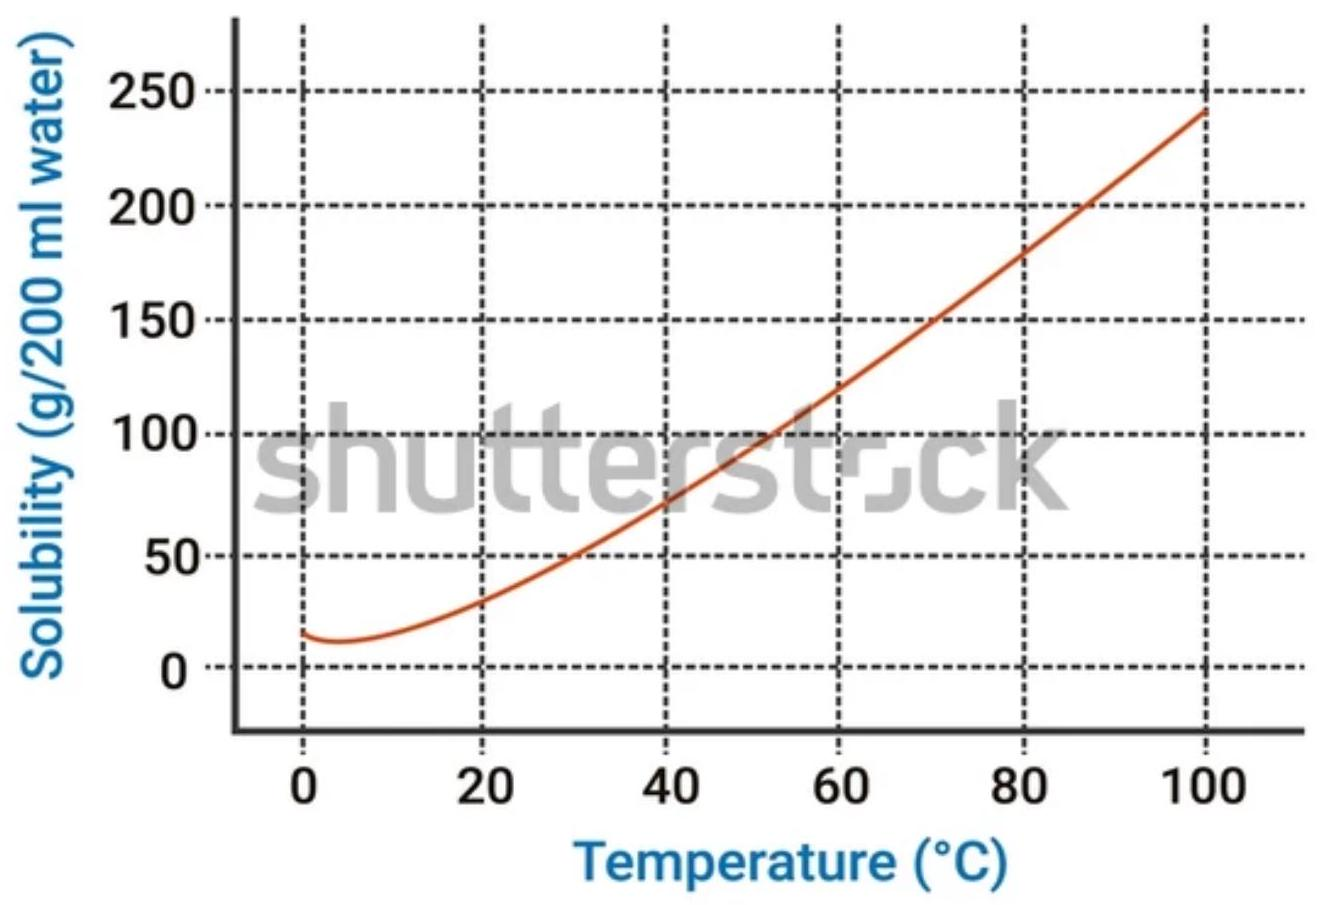
\includegraphics[width=0.6\textwidth]{2023_06_07_d6ea23c48f19fc3f50b0g-05}
\end{center}
\end{figure}

\section{Procedimiento experimental}
\subsection{Experimento 1}
\begin{figure}[H]
	\caption{Flujograma del procedimiento experimental $N^{\circ} 1$}
	\begin{center}
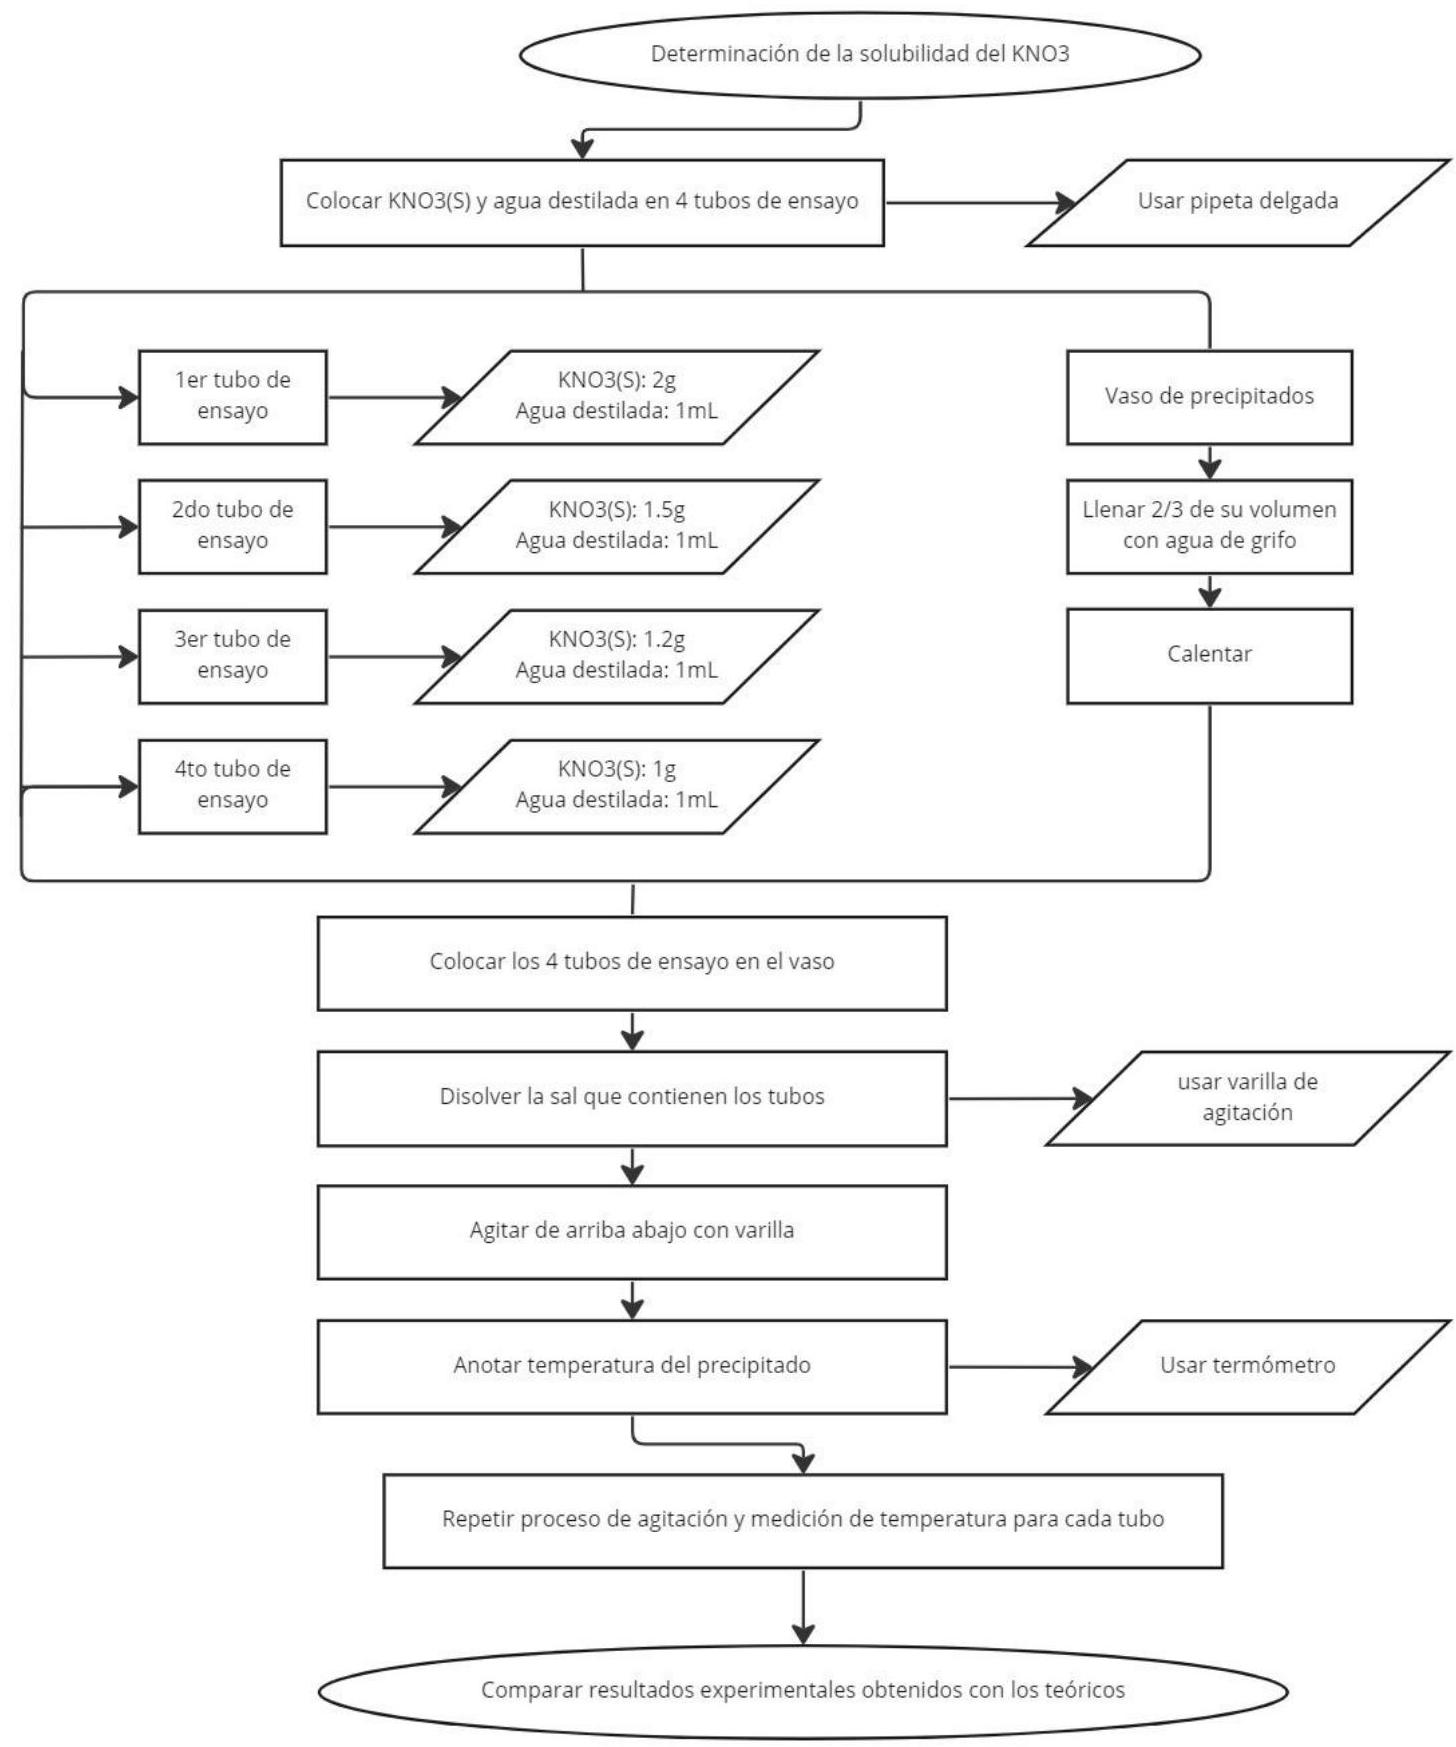
\includegraphics[width=0.8\textwidth]{2023_06_07_d6ea23c48f19fc3f50b0g-06}
\end{center}
\end{figure}

\subsection{Experimento 2}
\begin{figure}[H]
	\caption{Flujograma del procedimiento experimental $N^{\circ} 2$}
\begin{center}
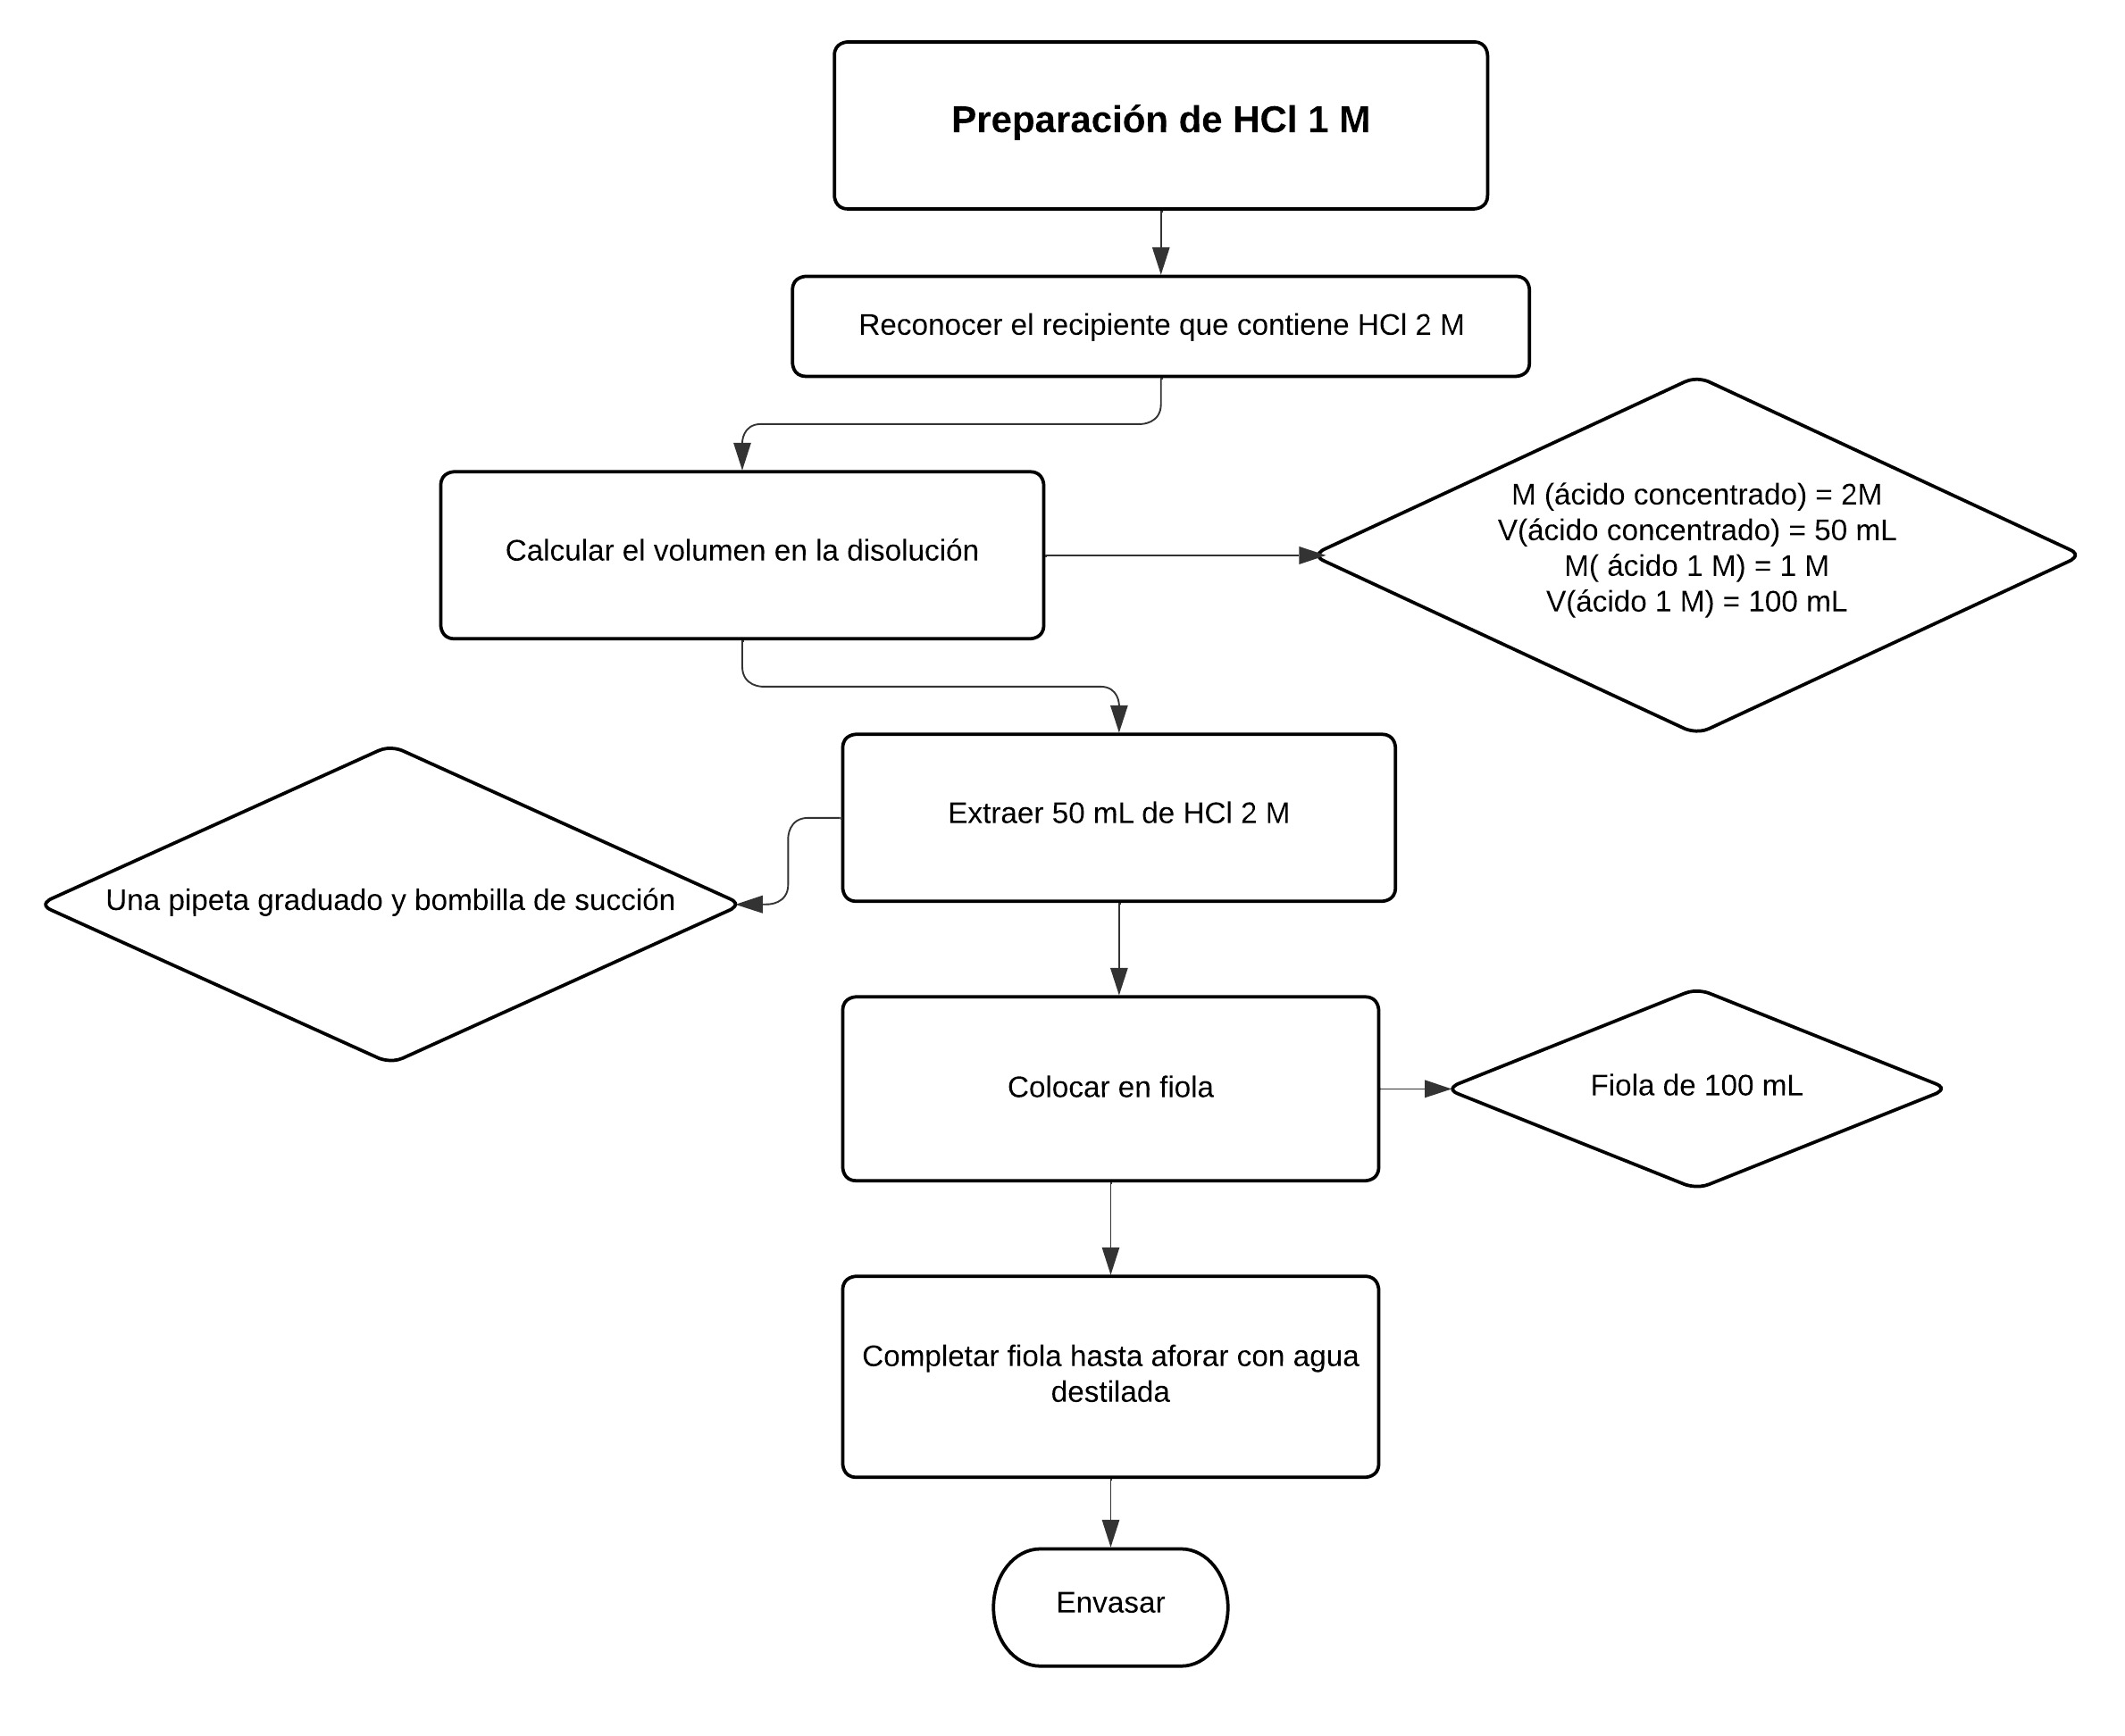
\includegraphics[width=0.7\textwidth]{diagramaexp2.jpg}
\end{center}
\end{figure}

\subsection{Experimento 3}

\begin{figure}[H]
	\caption{Flujograma del procedimiento experimental $N^{\circ} 3$}
\begin{center}
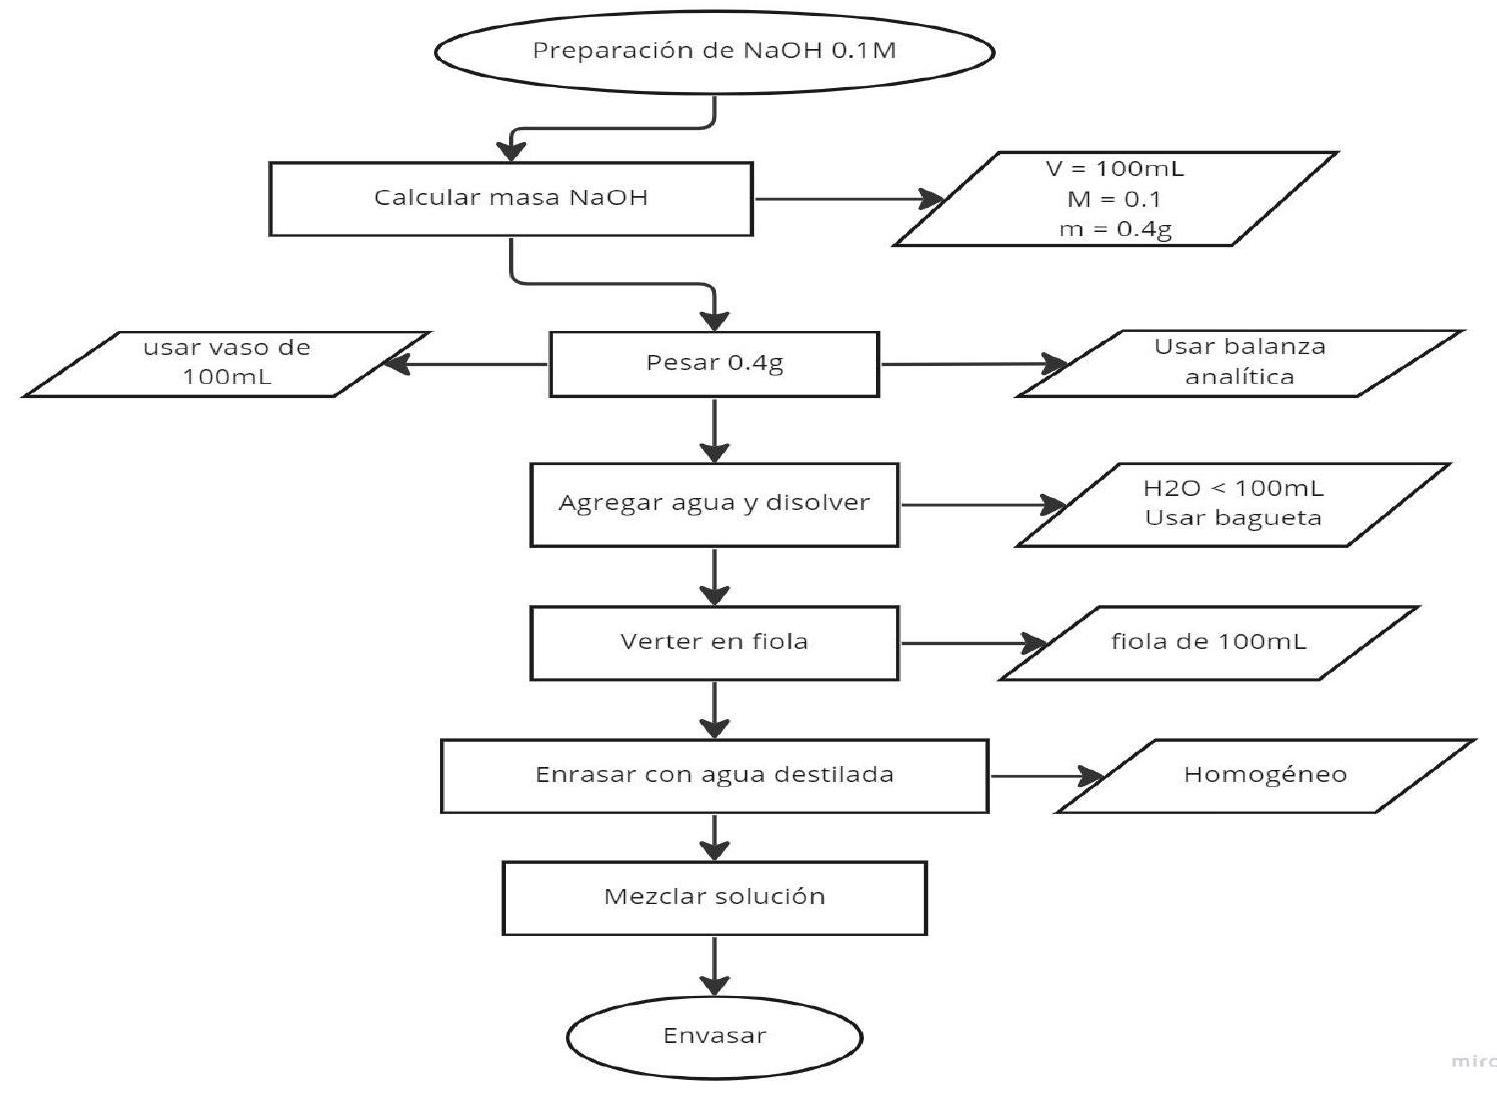
\includegraphics[width=0.7\textwidth]{2023_06_07_d6ea23c48f19fc3f50b0g-07(1)}
\end{center}
\end{figure}

\section{C\'alculos}
\subsection*{Experimento 1}


\begin{table}[H]
	\caption{ Datos experimentales de temperatura de aparición de cristales}
\begin{center}
\begin{tabular}{|c|c|c|}
\hline
Tubo de ensayo & Masa de KNO3 & $\mathbf{T}^{\circ}$ aparece precipitado \\
\hline
$\mathbf{1}$ & $2 \mathrm{~g}$ & $75^{\circ} \mathrm{C}$ \\
\hline
$\mathbf{2}$ & $1.5 \mathrm{~g}$ & $68^{\circ} \mathrm{C}$ \\
\hline
$\mathbf{3}$ & $1.2 \mathrm{~g}$ & $61^{\circ} \mathrm{C}$ \\
\hline
$\mathbf{4}$ & $1 \mathrm{~g}$ & $54^{\circ} \mathrm{C}$ \\
\hline
\end{tabular}
\end{center}
\end{table}

\begin{table}[H]
	\caption{ Cálculo de solubilidad para cada tubo de ensayo}
\begin{center}
\begin{tabular}{|l|l|l|l|}
\hline
Tubo de ensayo & $\begin{array}{l}\text { Masa } \\ \text { soluto(KNO3) }\end{array}$ & $\begin{array}{l}\text { Disolvente(Agua } \\ \text { destilada) }\end{array}$ & Solubilidad \\
\hline
1 & $200 \mathrm{~g}$ & $100 \mathrm{ml}$ & $200 \mathrm{~g} / 100 \mathrm{ml}$ \\
\hline
2 & $150 \mathrm{~g}$ & $100 \mathrm{ml}$ & $150 \mathrm{~g} / 100 \mathrm{ml}$ \\
\hline
3 & $120 \mathrm{~g}$ & $100 \mathrm{ml}$ & $120 \mathrm{~g} / 100 \mathrm{ml}$ \\
\hline
4 & $100 \mathrm{~g}$ & $100 \mathrm{ml}$ & $100 \mathrm{~g} / 100 \mathrm{ml}$ \\
\hline
\end{tabular}
\end{center}
\end{table}


\begin{figure}[H]
	\caption{Solubilidad Vs Temperatura de algunos compuestos i\'onicos Fuente. Chang, R., \& Godlsby, K(2017)}
\begin{center}
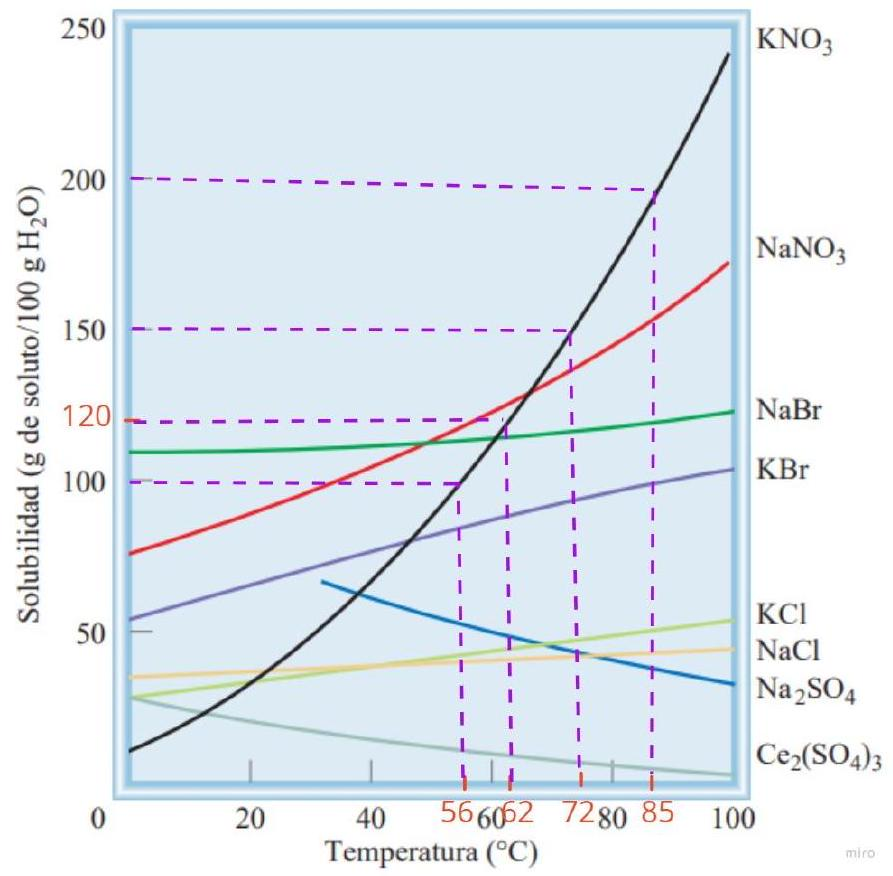
\includegraphics[ width=0.5\textwidth]{2023_06_07_d6ea23c48f19fc3f50b0g-08}
\end{center}
\end{figure}
Temperatura de precipitado te\'orico por la gr\'afica Solubilidad Vs Temperatura.
\[
	\text{Tubo 1}: 85^{\circ} \mathrm{C}
\]
\[
	\text{Tubo 2}: 72^{\circ} \mathrm{C}
\]
\[
	\text{Tubo 3}: 62^{\circ} \mathrm{C}
\]
\[
	\text{Tubo 4}: 56^{\circ} \mathrm{C}
\]
\begin{equation}
	\% \text{Error} =\dfrac{\mid \text { Teórico-Experimental } \mid}{\text { Teórico }} \times 100
\end{equation}


Tubo 1: \% Error $=\dfrac{|85-75|}{85} \times 100=11.8 \%$

Tubo 2: \% Error $=\dfrac{|72-68|}{72} \times 100=5.6 \%$

Tubo 3: \% Error $=\dfrac{|162-61|}{62} \times 100=1.6 \%$

Tubo 4: \% Error $=\dfrac{|56-54|}{56} \times 100=3.6 \%$

\subsection{Experimento 2}

$$
V_{\text {ácido concentrado }} x M_{\text {ácido concentrado }}=V_{\text {ácido 0.1M }} x M_{\text {ácido } 0.1 M}
$$

$$
\begin{gathered}
\mathrm{V} \times 2 \mathrm{M}=100 \mathrm{ml} \times 0.1 \mathrm{M} \\
\mathrm{V}=5 \mathrm{ml} \operatorname{HCl}(2 \mathrm{M})
\end{gathered}
$$

\subsection{Experimento 3}
\[
 n_{s t o}=\mathrm{M} \times V_{\text {sol }} 
\] 
\[
n_{s t o}  =0.1 \times 0.1 
\]
\[
n_{s t o}  =0.01 \operatorname{mol}(\mathrm{NaOH}) 
\]
\[
m_{\text {sto }}  =n_{\text {sto }} \times \bar{M}=0.01 \mathrm{~mol} \times 40 \mathrm{~g} / \mathrm{mol}=0.4 \mathrm{~g}(\mathrm{NaOH})
\]

\section{Resultados}
\subsection{Experimento 1}
\begin{table}[H]
\caption{Porcentaje de error obtenido para las temperaturas de precipitación}
\begin{center}
\begin{tabular}{|c|c|c|c|}
\hline
Tubo & $\mathbf{T}^{\circ}$ Teórica $\left({ }^{\circ} \mathbf{C}\right)$ & $\mathbf{T}^{\circ}$ Experimental $\left({ }^{\circ} \mathbf{C}\right)$ & Error (\%) \\
\hline
1 & 85 & 75 & 11.8 \\
\hline
2 & 72 & 68 & 5.6 \\
\hline
\end{tabular}
\end{center}
\end{table}

\begin{center}
\begin{tabular}{|l|l|l|l|}
\hline
3 & 62 & 61 & 1.6 \\
\hline
4 & 56 & 54 & 3.6 \\
\hline
\end{tabular}
\end{center}

\subsection{Experimento 2}
\[
\mathrm{V}=5 \mathrm{ml} \mathrm{HCl}(2 \mathrm{M})
\]

\begin{figure}[H]
\caption{HCl + $H{_2}O$}
\begin{center}
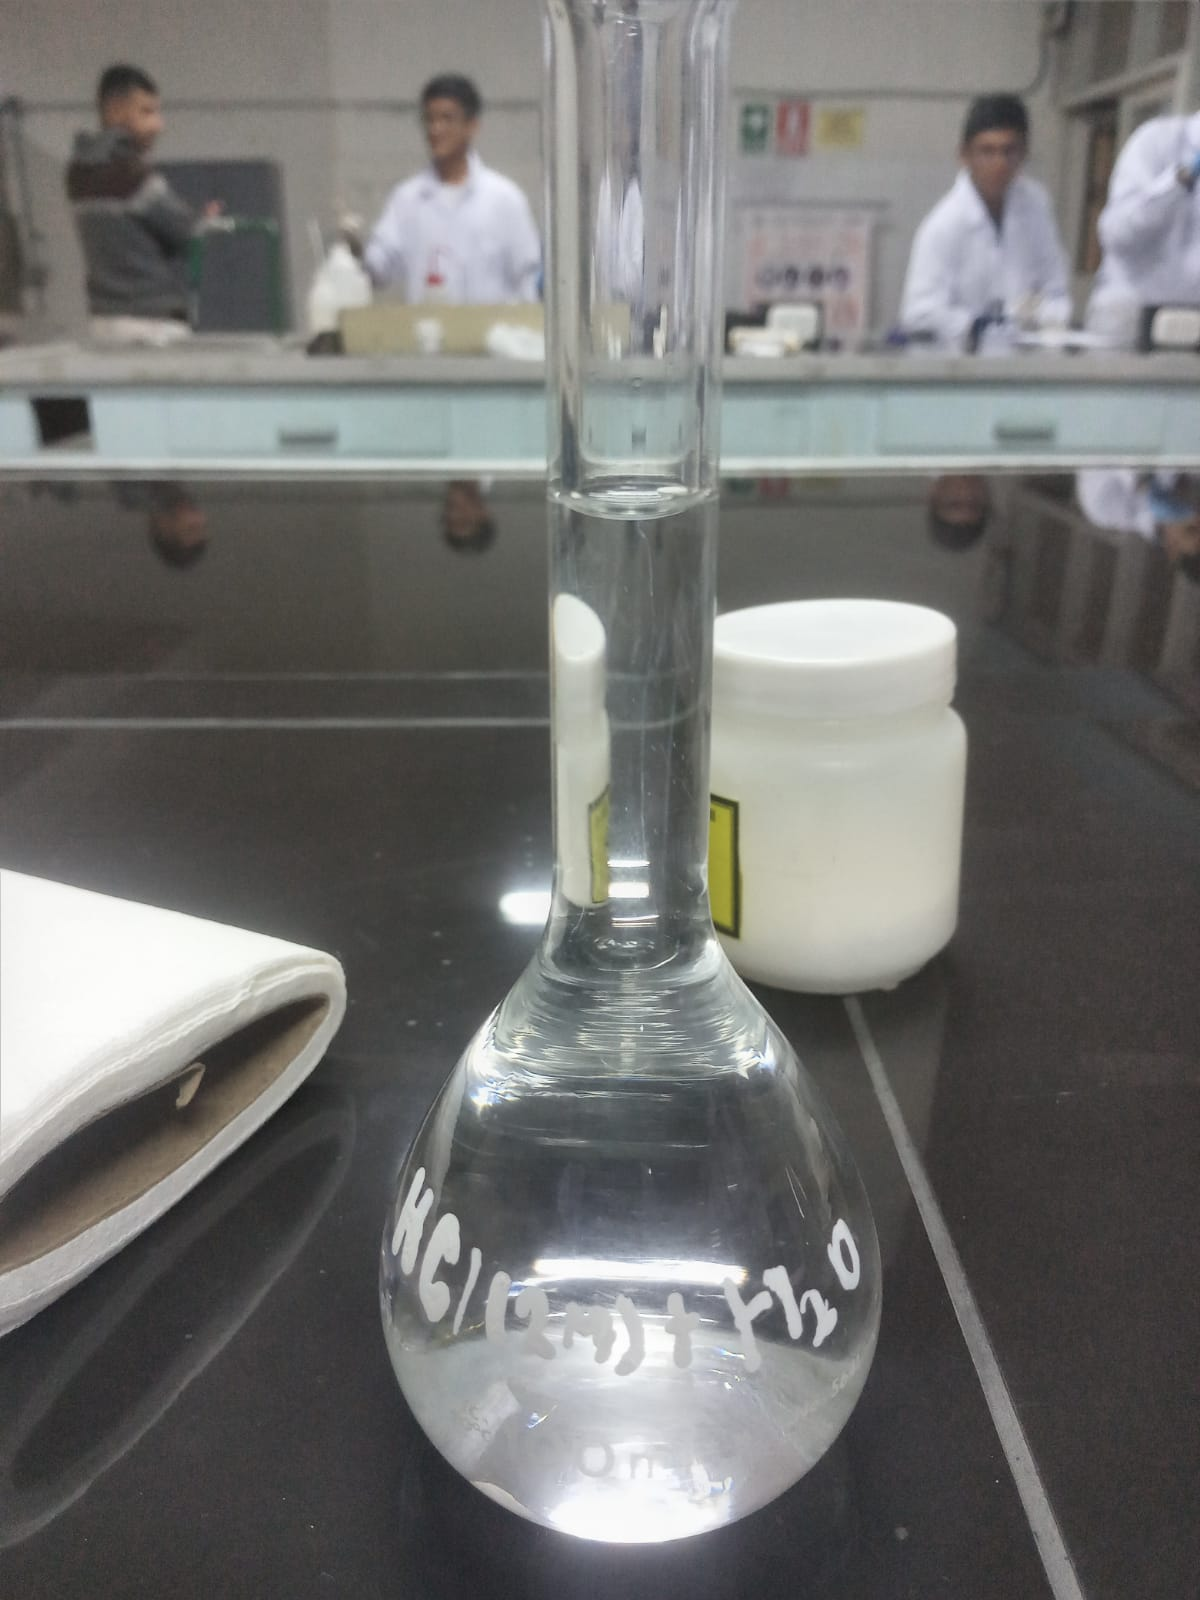
\includegraphics[ width=0.5\textwidth]{hcl.jpg}
\end{center}
\end{figure}

\subsection{Experimento 3}

\begin{table}[H]
\caption{Masa de NaOH obtenida para una concentración de $0.1 \mathrm{M}$}
\begin{center}
\begin{tabular}{|l|c|}
\hline
Volumen de solución (L) & 0.1 \\
\hline
Molaridad (mol/L) & 0.1 \\
\hline
Fórmula del soluto & $\mathrm{n}$ sto = M x Vsol \\
\hline
Masa molar del soluto $(\mathrm{g} / \mathrm{mol})$ & 40 \\
\hline
Masa de soluto a PESAR (g) & 0.4 \\
\hline
\end{tabular}
\end{center}
\end{table}


\begin{figure}[H]
\caption{NaOH + $H{_2}O$}
\begin{center}
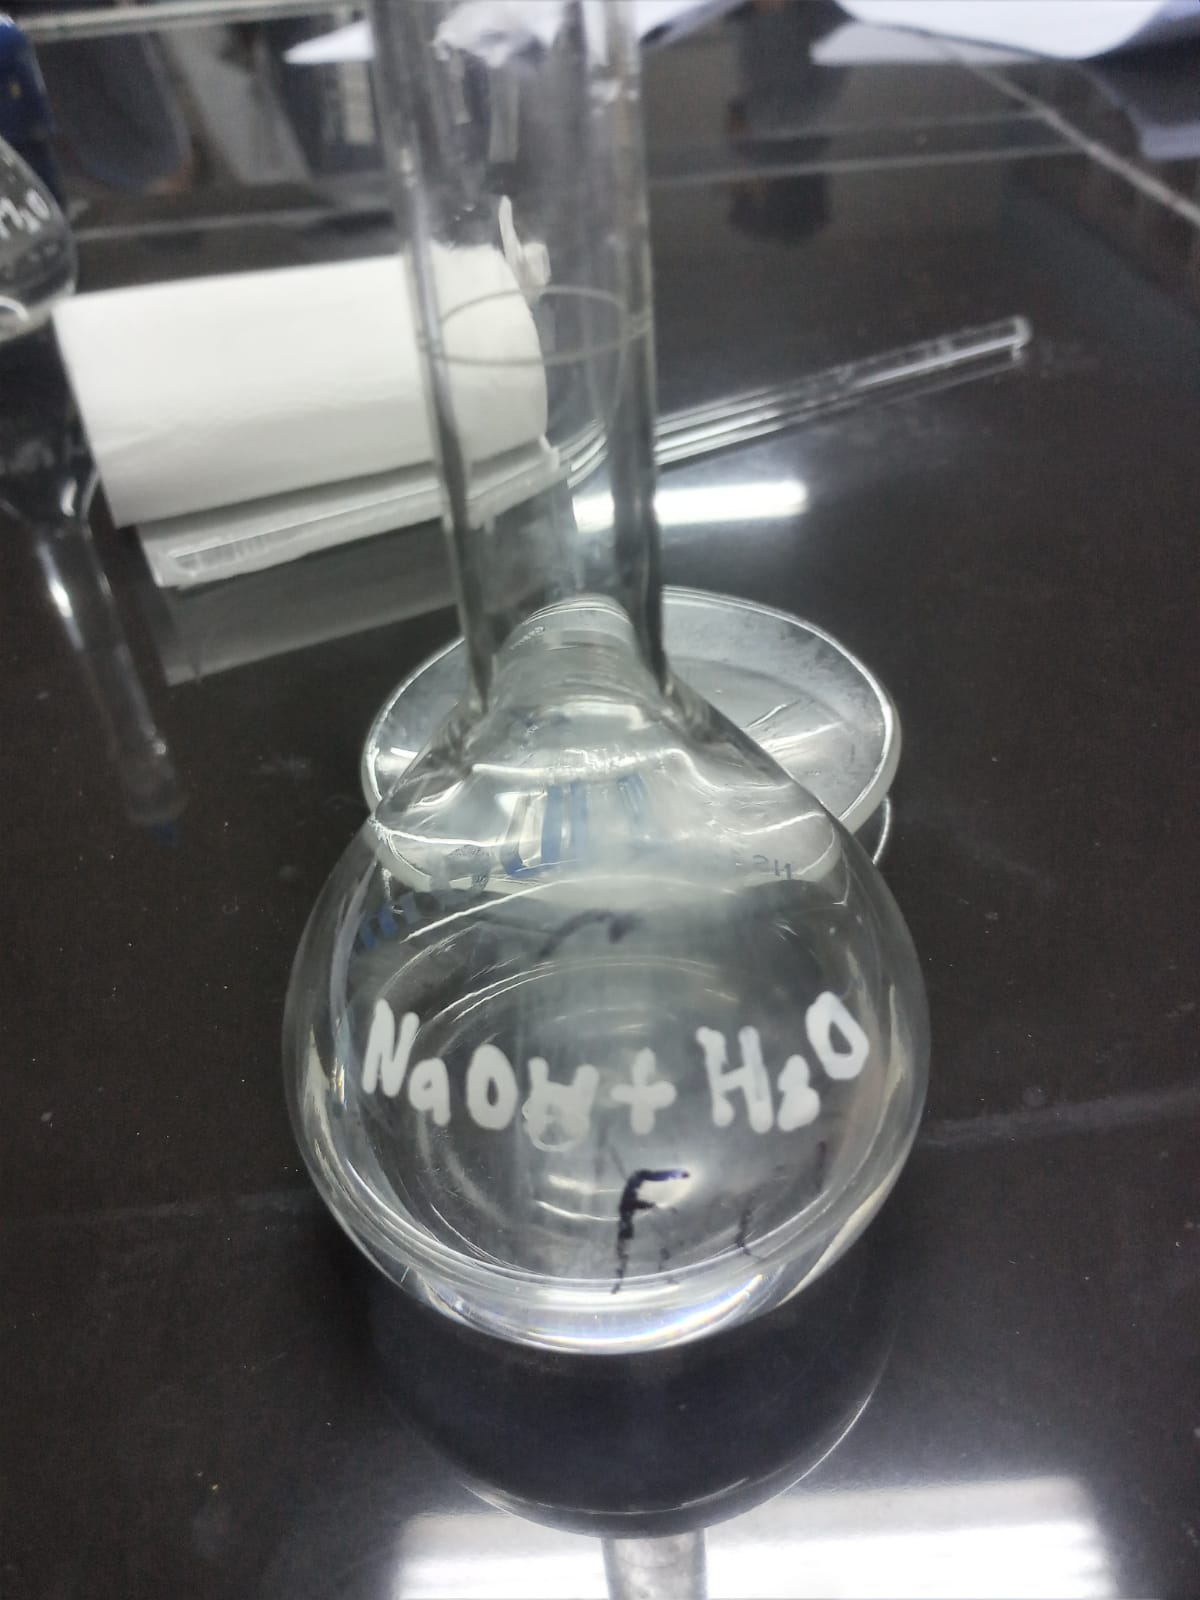
\includegraphics[ width=0.5\textwidth]{naohh2o.jpg}
\end{center}
\end{figure}

\section{Discusión de resultados}
\begin{itemize}
  \item Durante el desarrollo del primer experimento, al momento de colocar el $K N O_{3(S)}$ en los tubos de ensayo hubo pequeñas pérdidas de muestra, un evento que bien podría generar porcentaje de error; además, se pudo apreciar que el tubo 1 con $2 \mathrm{~g}$ de $K N O_{3(S)}$ fue el primero en cristalizarse, de esta manera se pudo notar que a mayor muestra de $\mathrm{KNO}_{3(S)}$ más rápido se daba su cristalización. Esto se debe a que el tubo con mayor concentración se sobresaturó antes que los de menor concentración y esta relación la pudimos notar en la curva de saturación para el $\mathrm{KNO}_{3(S)}$. Así mismo, la parte sobresaturada se pudo observar en la cristalización, ya que la solución ya no pudo contener cierta cantidad de soluto y por eso se vio la precipitación en forma de cristales.


  \item Debido a que el $K_{2} O_{3}$ disuelto en agua presentan interacciones ión-dipolo en la mezcla y presenta momento dipolar los iones del compuesto $\mathrm{KNO}_{3}$ pueden solvatar, es decir, sus iones rodearse de moléculas del disolvente que al ser agua se llama hidratación. La solvatación de los iones se dará solo si la energía para producirla es compensada con la separación de los iones del compuesto. En nuestro experimento se pudo observar se da la disolución del $\mathrm{KNO}_{3}$ en agua, por lo que se cumple lo mencionado.

\end{itemize}
\section{Conclusiones}
\begin{itemize}
	\item  Se observó que en la gráfica de solubilidad, mientras la concentración de la solubilidad de $KNO_3$ aumentaba también lo hacía la temperatura de cristalización
	\item  Los porcentajes de error obtenidos en las temperaturas de cristalización de los cuatro tubos no fueron mayores al $11.8\%$, ya que se tuvo mucha atención al observar las temperaturas de cristalización. Sin embargo se podría mejorar la detección de la temperatura si los experimentadores están mucho más cerca de los tubos, ya que los cristales aparecen repentinamente y la lectura de la temperatura es muy rápida, ya que esta disminuye rápidamente.
	\item  El volumen de ácido de HCl usado en la preparación fue de 5 mL, el cual es mucho menor a los 100 mL utilizados, ya que la concentración es mucho mayor al de la preparación obtenida.
	\item  La masa de NaOH(0.1M) para 100 mL fue de 0.4 g
\end{itemize}	
\begin{thebibliography}{99}

\bibitem{chang2005quimica}
Chang, Raymond.
\textit{Química}.
McGraw-Hill, 2005.
\bibitem{UNI}
Universidad Nacional de Ingieneria.
\textit{Manual de Laboratorio}.
2023.

\end{thebibliography}
\end{document}
